\documentclass[12pt]{article}
\usepackage{xeCJK}
\usepackage{amsmath}
\usepackage{pdfpages}
\usepackage[colorlinks,linkcolor=red]{hyperref}

\title{Project 1}
\author{
李林翼 \footnote{计43, 2014011361, limyik.li96@gmail.com}
\ 朱祺 \footnote{计43, 2014011336, zhu-q14@mails.tsinghua.edu.cn}
}
\begin{document}
\maketitle{}
\tableofcontents
\newpage

\section{数据预处理和可视化}
\subsection{新闻数据读入与建立数据框对象}
第一步是数据的读取。此处为了后面便于处理,将读取的数据持久化,保存为 result/data.csv 文件。
可以分为以下三步:确定要读取的新闻的属性;读取新闻到data.frame;保存为 .csv 文件。
\subsubsection{确定要读取的新闻的属性}
根据proj1的要求和new\_york\_times\_annotated\_corpus.pdf文件,选定以下属性读取:
\begin{description}
  \item[docid]
  新闻唯一标识符,也是文档的名字
  \item[title]
  新闻的标题
  \item[categories]
  新闻的类别,使用online\_sections属性。例子:``Business; Technology''。
  \item[locations]
  新闻中提到的地点,使用Locations和Online\_Locations属性。例子:``NEW YORK, NY''。
  \item[day\_of\_month,month,year]
  发行日期,使用publication\_*属性。例子:26; 06; 1995。
  \item[publication\_date]
  发行日期,使用Publication Date属性。例子:19950627T000000。
  \item[body]
  新闻正文。
\end{description}
\subsubsection{读取新闻到data.frame}
这一部分主要的函数readDoc()在readDoc.R中。使用了XML和stringr两个库辅助处理。
属性不存在时标记为NA。
\subsubsection{数据持久化}
主要的函数readAll()和extractAll()在readDoc.R中。读取目录下所有新闻,将data.frame写入
data.csv

\subsection{对新闻全文进行预处理}
tm库中有很方便的函数可以进行预处理,包括去除标点符号、停用词、数字、空白字符,将
大写字母都转化为小写,以及词干化处理。所有的这些处理都可以使用tm\_map()函数,
通过map的方式将转化函数应用到每一个文档语料上。主要函数getCorpus()在process.R中,返回Corpus。
\subsection{将新闻表示成BagOfWords向量}
利用上一步得到的Corpus,借助DocumentTermMatrix函数,可以得到文档-词条矩阵,
每一行即是BagOfWords向量。
\subsection{筛选出出现次数大于100的词并画 wordcloud}
DocumentTermMatrix得到的文档-词条矩阵通过findFreqTerms函数找出出现次数大于100的词。
利用wordcloud函数绘制云图。实现在process.R的drawWordCloud()中。结果见\ref{fig:wordCloud}。
\begin{figure}[htbp]
\centering
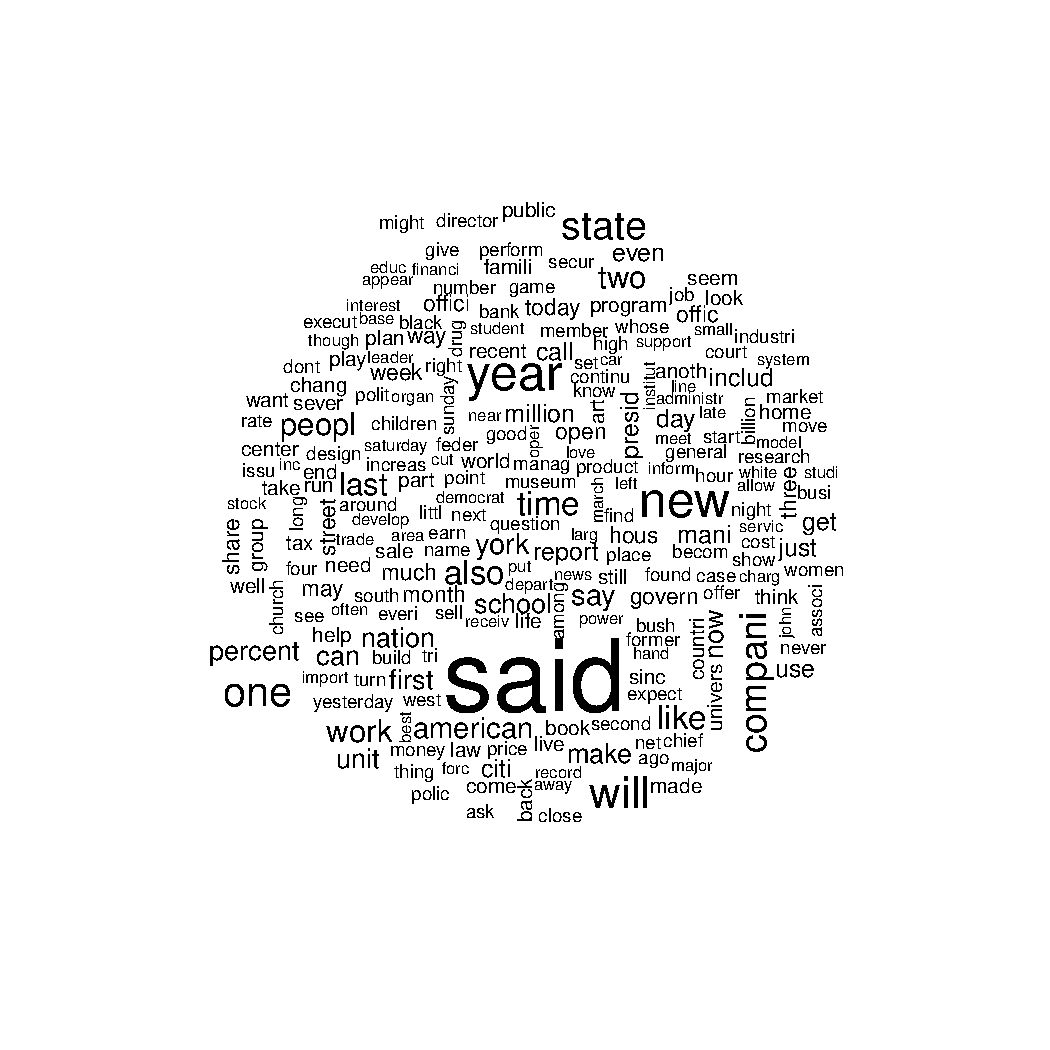
\includegraphics[width=1.0\textwidth]{../result/wordCloud.pdf}
\caption{wordCloud}
\label{fig:wordCloud}
\end{figure}
出现最多的词是said,挺符合新闻报道的特点的。其他高频词如state、compani、school、work、peopl、
american还是很合理的。但也有些没什么实际含义的词如also、dont、next、get、just。

\subsection{画出单词长度的分布直方图}
与上类似,findFreqTerms(DocumentTermMatrix(corpus), 0)得到所有word,按单词长度统计。
利用qplot画图。实现在process.R的drawWordLength()中。结果见\ref{fig:wordLength}。
\begin{figure}[htbp]
\centering
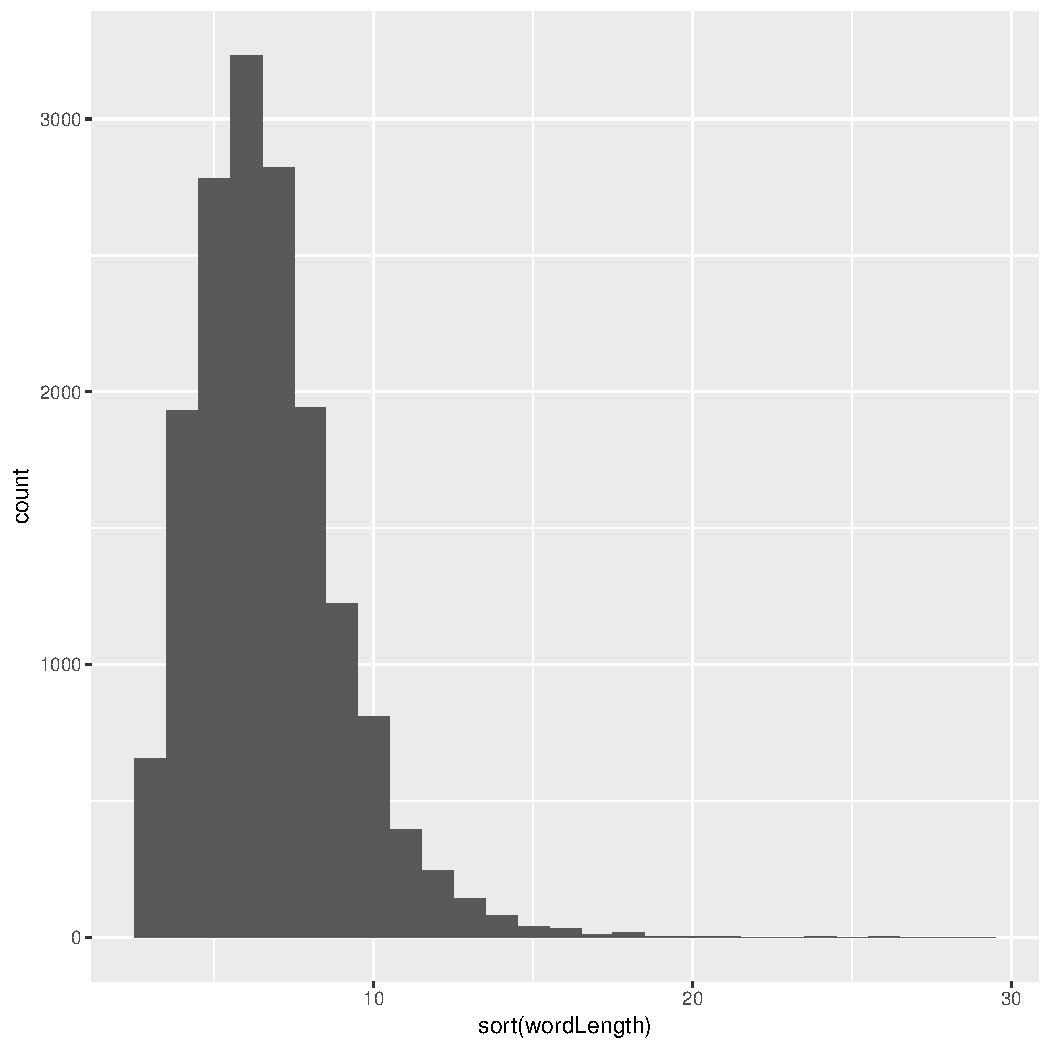
\includegraphics[width=1.0\textwidth]{../result/wordLength.pdf}
\caption{wordLength}
\label{fig:wordLength}
\end{figure}
可以看到单词的长度基本上在10以内,主要集中在3-6个字母之间。

\subsection{画出新闻类别的分布直方图}
\subsection{画出每个月新闻数量的分布直方图}


\section{新闻相似度计算}
\subsection{计算新闻之间的余弦相似度矩阵}
\subsection{计算类别内新闻之间的平均相似度}
\subsection{计算两个类别的新闻之间的平均相似度}

\section{扩展分析}

\end{document}  

